\section{Experiments}
\label{sec:eval}

We evaluate the proposed method on two benchmark tasks: (i) cart-pole swing-up and (ii) truck backer-upper.
For the cart-pole swing-up task, the initial pole angle $\phi$ is sampled uniformly from $[145^\circ, 215^\circ]$, where $\phi = 0^\circ$ corresponds to the upright position.
For the truck backer-upper task, the initial $x$ and $y$ positions are sampled uniformly from $[15, 20]$ and $[-10, 10]$, respectively. The trailer and truck orientations are drawn uniformly from $[-90^\circ, 90^\circ]$, with the goal of backing the trailer to the position $(x,y)=(0,0)$.
Detailed simulation and controller settings for these tasks can be found in~\cite{arXiv26_Walker_IFAC,walkerSampleefficientSmoothCrossentropy2026}.
To assess the method beyond these classical tasks, we additionally consider (iii) CheetahRun and (iv) WalkerRun from MuJoCo Playground~\cite{zakkaDemonstratingMuJoCoPlayground2025} as supplementary validation.

We first analyze the effect of the trust region parameters and the proposal-update behavior, including the entropy lower bound, before comparing the resulting method against heuristic \ac{MPPI}-like baselines.
As baseline, we use an \ac{MPPI}-like method from~\cite{arXiv26_Walker_IFAC}, which also updates proposal mean and covariance from weighted samples but does not enforce a trust region. Instead, it relies on a temperature heuristic~\cite{pezzatoSamplingbasedModelPredictive2025} and momentum-style smoothing~\cref{eq:cem_momentum_mean} to stabilize optimization.

To isolate the effect of the trust region formulation, both methods use the same algorithmic enhancements from \cref{sec:alg_improvements} and the same hyperparameters as in~\cite{arXiv26_Walker_IFAC}.
We compare performance in terms of sample efficiency, smoothness of the control inputs, and convergence over iterations.
Smoothness is measured using $\sum_{k=1}^{T-1} \| \vu_{k} - \vu_{k-1} \|^2 $, where $T$ is the number of time steps in a simulation (see~\cite{arXiv26_Walker_IFAC}), and a lower value indicates a smoother control trajectory.
Both sample efficiency and convergence are evaluated in terms of cumulative cost, which is the sum of stage costs over $T$ steps.

We consider four sampling methods: random sampling, low-discrepancy sampling (Sobol~\cite{joeConstructingSobolSequences2008} and Halton~\cite{owen2017randomizedhaltonalgorithmr}), and the deterministic \ac{LCD}-based sampling. 
To transform the uniform Sobol and Halton samples to an arbitrary Gaussian, we use the inverse transform and eigenvalue decomposition, as described in~\cite{frischGeneralizedFibonacciGrid2023}, with no further moment correction.
In the plots, heuristic baseline variants are shown with solid lines, and trust region variants are shown with dashed lines labeled with suffix \emph{TR}. 
Labels indicate the sampling method, where the prefix \emph{ds} denotes deterministic \ac{LCD} sampling. 
% Trust region variants are denoted by the suffix \emph{TR}.
Furthermore, we compare to the \ac{CEM} using \ac{LCD}-based samples~\cite{walkerSampleefficientSmoothCrossentropy2026} denoted by \emph{dsCEM}.

Each method and setting is evaluated over \num{100} runs, and statistics are reported as median and interquartile range. 
% Since Sobol and Halton show very similar trends, we present Halton only in the main plots for readability. 
Results are shown in \cref{fig:cart_pole:results,fig:truck:results,fig:eps_sweep}.



\subsection{Trust Region Parameter Sensitivity and Proposal Behavior}

\begin{figure}
    \centering
    % \begin{subfigure}{\columnwidth}
        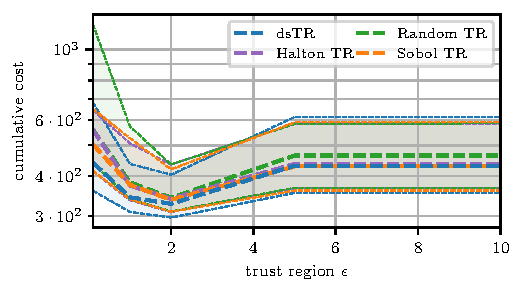
\includegraphics[width=\linewidth]{images/cart_pole/cumulative_costs_vs_trust_region_eps_N_100_iter_5_log.pdf}%
    %     \caption{Cart-pole swing-up}%
    %     \label{fig:cart_pole:eps_sweep}%
    % \end{subfigure}
    % \begin{subfigure}{\columnwidth}
    %     \centering%
    %     %\includegraphics[width=\linewidth]{images/truck/cumulative_costs_eps_sweep_iter_3_me_-50.0_log.pdf}%
    %     \caption{Truck backer-upper}%
    %     \label{fig:truck:eps_sweep}%
    % \end{subfigure}
    \caption{Cumulative costs over trust region parameter $\epsilon$ for the cart-pole swing-up environment.
    }
    \label{fig:eps_sweep}%
\end{figure}

The $\epsilon$-sweep result for the proposed trust region method with random, low-discrepancy, and deterministic \ac{LCD} sampling is shown in \cref{fig:eps_sweep} for \num{100} samples and \num{5} optimizer iterations, exemplified for cart-pole swing-up.
The lowest cumulative cost is achieved at $\epsilon = 2$ for all sampling methods.
If $\epsilon$ is larger, the trust region constraint is looser and allows for more aggressive updates that can lead to worse performance. 
When $\epsilon$ is smaller, the trust region constraint is tighter, which can lead to more conservative updates requiring more iterations to achieve good performance.
However, if large iteration counts are feasible, a smaller $\epsilon$ can achieve better performance.

The entropy lower bound $H_{\min}$ has little effect in the settings considered in the main benchmark comparisons, where the proposal does not collapse within the feasible iteration counts. 
However, for longer optimization runs, $H_{\min}$ prevents premature collapse of the proposal and preserves exploration, as shown in \cref{fig:cart_pole:100step}. Without the entropy constraint, the proposal collapses and fails to reach the global minimum; with the entropy constraint, it retains sufficient exploration to converge toward the optimum.

\begin{figure}%
    \centering%
    \begin{subfigure}{0.48\columnwidth}
        % trim =left bottom right top
        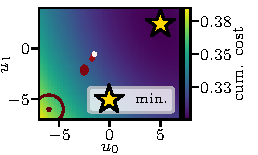
\includegraphics[, trim=0 0 1.3cm 0.0cm, clip]{images/proposal_convergence/proposal_convergence_dscem_cbar_cost.pdf}%
        \caption{dsCEM}%
        \label{fig:cart_pole:100step:dscem}%
    \end{subfigure}
    \begin{subfigure}{0.48\columnwidth}
        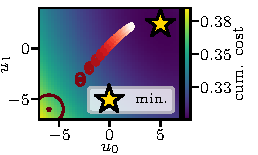
\includegraphics[, trim=0 0 0 0.0cm, clip]{images/proposal_convergence/proposal_convergence_dsmppi_cbar_cost.pdf}%
        \caption{dsMPPI}%
        \label{fig:cart_pole:100step:dsmppi}%
    \end{subfigure}
    \\
    \begin{subfigure}{0.48\columnwidth}
        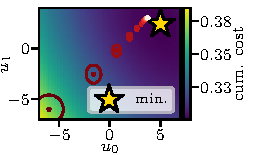
\includegraphics[, trim=0 0 1.3cm 0.0cm, clip]{images/proposal_convergence/proposal_convergence_dstr_no_entropy_constraint_cbar_cost.pdf}%
        \caption{dsTR (no entropy constraint)}%
        \label{fig:cart_pole:100step:dstr_no_entropy}%
    \end{subfigure}
    \begin{subfigure}{0.48\columnwidth}
        \centering%
        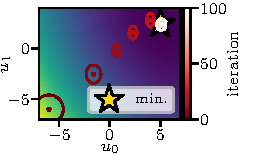
\includegraphics[, trim=0 0 0 0.0cm, clip]{images/proposal_convergence/proposal_convergence_dstr_entropy_constrained_cbar_iter.pdf}%
        \caption{dsTR (entropy constrained)}%
        \label{fig:cart_pole:100step:dstr_entropy_constrained}%
    \end{subfigure}    
    \caption{Convergence of a single cart-pole control step with $\horizon=\num{2}$ ($\vxi=[u_1,u_2]\T$), $\epsilon=2$, and $H_{\min}=0$ for the pathological case where the initial proposal is far from $\min J(\vxi)$. Gaussian proposals with diagonal covariance are shown as $2\sigma$ ellipses over \num{100} iterations; every 10th iterate is plotted and color indicates the iteration number. Without the entropy constraint (a--c), the proposal collapses prematurely; with it, it retains exploration and converges to the optimum.
    }
    \label{fig:cart_pole:100step}%
\end{figure}%

For the main comparisons, the trust region parameters are fixed to $\epsilon = 2$ and $H_{\min} = -50$.
Since Sobol and Halton samples show very similar trends, we present Sobol only in the following plots for readability.

\begin{figure}%
    \centering%
    \begin{subfigure}{\columnwidth}
        % trim =left bottom right top
        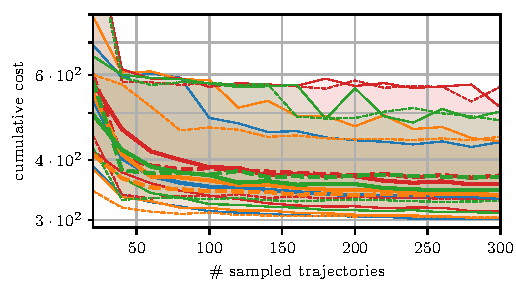
\includegraphics[width=\linewidth,trim=0 0 0.05cm 0.1cm, clip]{images/cart_pole/cumulative_costs_eps_2.0_iter_3_me_-50.0_log_wo_legend.pdf}%
        \caption{Cumulative costs over sample size}%
        \label{fig:cart_pole:cum_cost}%
    \end{subfigure}
    \begin{subfigure}{\columnwidth}
        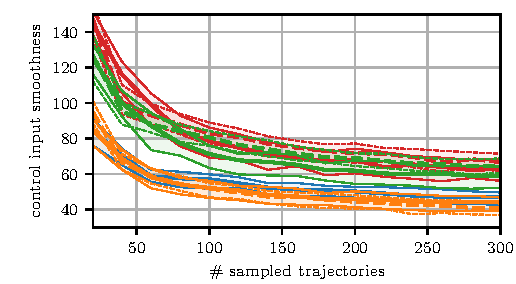
\includegraphics[width=\linewidth,trim=0 0 0.05cm 0.1cm, clip]{images/cart_pole/action_smoothness_eps_2.0_iter_3_me_-50.0_wo_legend.pdf}%
        \caption{Control input smoothness}%
        \label{fig:cart_pole:action_smoothness}%
    \end{subfigure}
    \begin{subfigure}{\columnwidth}
        \centering%
        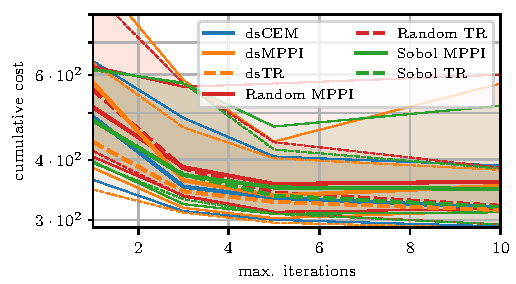
\includegraphics[width=\linewidth, ,trim=0 0 0.05cm 0.1cm, clip]{images/cart_pole/cumulative_costs_vs_max_iter_N_100_eps2.0_log.pdf}%
        \caption{Cumulative costs over optimizer iterations}%
        \label{fig:cart_pole:convergence}%
    \end{subfigure}    
    \caption{Results for the cart-pole swing-up environment. All plots share the same legend.
    }
    \label{fig:cart_pole:results}%
\end{figure}%


\begin{figure}%
    \centering%
    \begin{subfigure}{\columnwidth}
        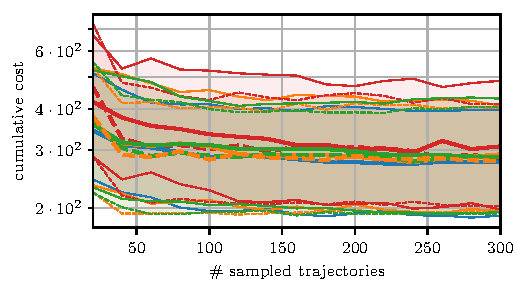
\includegraphics[width=\linewidth]{images/truck/cumulative_costs_eps_2.0_iter_3_me_-50.0_log_wo_legend.pdf}%
        \caption{Cumulative costs over sample size}%
        \label{fig:truck:cum_cost}%
    \end{subfigure}
    \begin{subfigure}{\columnwidth}
        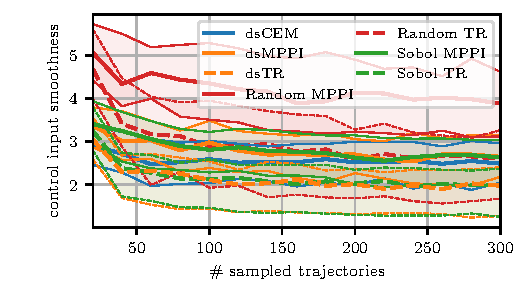
\includegraphics[width=\linewidth]{images/truck/action_smoothness_eps_2.0_iter_3_me_-50.0.pdf}%
        \caption{Control input smoothness}%
        \label{fig:truck:action_smoothness}%
    \end{subfigure}
    \begin{subfigure}{\columnwidth}
        \centering%
        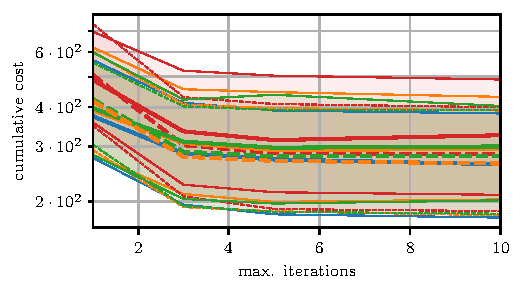
\includegraphics[width=\linewidth]{images/truck/cumulative_costs_vs_max_iter_N_100_eps2.0_log_wo_legend.pdf}%
        \caption{Cumulative costs over optimizer iterations}%
        \label{fig:truck:convergence}%
    \end{subfigure}    
    \caption{Results for the truck backer-upper environment.
    All plots share the same legend as in \cref{fig:cart_pole:results}.
    }
    \label{fig:truck:results}%
\end{figure}%

\subsection{Sample Efficiency}
\label{sec:eval:sample_efficiency}

In the sample-efficiency analysis, the number of optimizer iterations is fixed to three, and sample sizes from \num{20} to \num{300} are evaluated (see \cref{fig:cart_pole:cum_cost,fig:truck:cum_cost}).
%
In both environments, trust region variants mostly achieve lower cumulative costs than heuristic variants when the sample budget is small (e.g., $N \le 100$),  which indicates improved sample efficiency.
% A notable exception is Sobol sampling in cart-pole swing-up, where the heuristic variant is competitive at very low $N$.
%
Across settings, the trust region method with deterministic \ac{LCD} sampling consistently outperforms its heuristic counterpart and dsCEM.
This advantage is particularly pronounced for the cart-pole swing-up, where the proposed dsTR clearly achieves the best performance in the low-sample regime.

\subsection{Control Input Smoothness}
\label{sec:eval:smoothness}
The smoothness comparison, shown in \cref{fig:cart_pole:action_smoothness,fig:truck:action_smoothness}, uses the same sample and iteration settings as in \cref{sec:eval:sample_efficiency}.
%
In the truck backer-upper environment, trust region variants improve control-input smoothness over their heuristic counterparts at low sample sizes across all sampling strategies.
%
In cart-pole swing-up, heuristic variants with random and Sobol sampling are smoother than their corresponding trust region variants for most sample sizes.
For deterministic \ac{LCD} sampling, however, dsTR achieves slightly lower or equal smoothness values than dsMPPI and dsCEM in most settings.
%
Therefore, trust region updates do not necessarily improve smoothness, and their smoothness mainly depends on the sampling strategy.

\subsection{Convergence}

In the convergence analysis, displayed in \cref{fig:cart_pole:convergence,fig:truck:convergence}, the sample size is fixed to $N=100$, and the maximum number of iterations ($\numCEMIter$) is varied over $\{1,3,5,10\}$.
%
Trust region variants show faster convergence than heuristic variants and dsCEM, with lower median cumulative costs and tighter interquartile ranges across iterations.
This effect is particularly pronounced for the truck backer-upper: even after ten iterations, heuristic variants do not reach the cost achieved by trust region variants using only three iterations for any sampling strategy.
%
Across both environments, dsTR provides the best convergence behavior, achieving lower costs with fewer iterations than all alternatives.

\subsection{Runtime}

\begin{table}[t]
    \centering    
    \caption{Computation times per control step ($\numCEMIter=3$).}
    \label{tab:computation_times}
    \setlength{\tabcolsep}{2pt}
    {
    \small
    % set siunitx options for better readability
    \sisetup{round-mode=places,round-precision=1, scientific-notation=fixed, fixed-exponent=-3, drop-exponent=true}
    \begin{tabular}{lcc}
        \toprule
        Method      & Cart-Pole Swing-Up$^{\text{a}}$             & Truck Backer-Upper$^{\text{a}}$  
        \\
        \midrule
        dsMPPI      & $\num{0.1710} \pm \num{0.0469}$ & $\num{0.0691} \pm \num{0.0422}$
        \\
        dsTR        & $\num{0.2018} \pm \num{0.0557}$ & $\num{0.0836} \pm \num{0.0472}$                  
        \\
        Halton MPPI & $\num{0.1713} \pm \num{0.0414}$ & $\num{0.0806} \pm \num{0.0467}$
        \\
        Halton TR   & $\num{0.2086} \pm \num{0.0524}$ & $\num{0.0980} \pm \num{0.0530}$
        \\
        Sobol MPPI  & $\num{0.1840} \pm \num{0.0519}$ & $\num{0.0832} \pm \num{0.0473}$
        \\
        Sobol TR    & $\num{0.2118} \pm \num{0.0558}$ & $\num{0.0955} \pm \num{0.0517}$
        \\
        Random MPPI & $\num{0.1661} \pm \num{0.0488}$ & $\num{0.0645} \pm \num{0.0364}$
        \\
        Random TR   & $\num{0.1995} \pm \num{0.0504}$ & $\num{0.0789} \pm \num{0.0480}$
        \\
        dsCEM   & $\num{0.1669} \pm \num{0.0454}$ & $\num{0.0634} \pm \num{0.0358}$
        \\
        \bottomrule
        \multicolumn{3}{l}{\footnotesize $^{\text{a}}$mean $\pm$ standard deviation in \si{\milli\second} evaluated over 100 runs} \\
    \end{tabular}
    }
\end{table}

Computation times per control step are reported in \cref{tab:computation_times}.
% 
All runtimes were measured on a single Intel Xeon Platinum 8368 core.
As expected, heuristic variants are generally faster than trust region variants because trust region updates require an additional optimization step.
Across sampling methods, deterministic variants (dsTR and dsMPPI) are faster than low-discrepancy variants (Halton and Sobol) due to precomputed samples, while random sampling remains the fastest.
Further runtime reductions are possible through parallelization.

\subsection{MuJoCo Playground Validation}

As a supplementary validation beyond the classical benchmark tasks, we evaluate the method on WalkerRun and CheetahRun from MuJoCo Playground~\cite{zakkaDemonstratingMuJoCoPlayground2025}. 
The control discretization is $\SI{0.05}{\second}$, the simulation step is $\SI{0.01}{\second}$, and each run spans \num{250} simulation steps. 
We use $N=\num{100}$ samples, $\epsilon = \num{3}$, $H_{\min} = \num{-75}$, and a horizon length of $\horizon=10$. The initial proposal is a Gaussian $\Gaussian(\vzero, \mI)$, transformed with $\beta=1$ (see \cref{sec:standard_improvements}) to introduce temporal correlations; other controller settings match the previous experiments.
Both environments use six-dimensional control inputs, resulting in a 60-dimensional optimization vector over the horizon.
Each experiment is repeated for \num{100} randomized initial states.

\begin{figure}%
    \centering%
        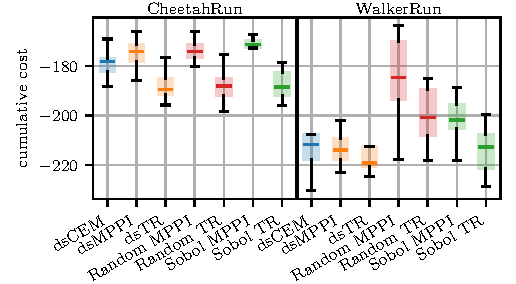
\includegraphics[width=\linewidth]{images/mujoco_playground_exp3/cumulative_costs_eps_3.0_iter_3_me_-75.0.pdf}
    \caption{MuJoCo Playground validation results.}
    \label{fig:mujoco}%
\end{figure}%

The results in \cref{fig:mujoco} are consistent with the benchmark study: trust-region variants outperform the heuristic baselines, and the deterministic \ac{LCD}-based trust-region method achieves the lowest median cost, with the largest improvement in WalkerRun.



\section{Discussion}
\label{sec:discussion}

The experiments show that trust region updates improve both sample efficiency and convergence compared to heuristic updates across all considered settings and sampling methods.
Although heuristic methods remain competitive in certain settings, the proposed trust region \ac{MPC} is consistently outperforming them, in particular, when computational budgets are limited, \ie, when only a small number of samples and iterations are feasible.
The entropy lower bound further serves as a safeguard against premature proposal collapse in longer optimization runs, where the proposal can otherwise contract too quickly and lose exploration before reaching the optimum.

Note that reducing the required sample size directly decreases computation time and memory usage. 
On parallel hardware, even a difference of a single sample can significantly affect the runtime. 
\Eg, if the hardware can process up to 32 trajectories (samples) in parallel, requiring 33 samples would effectively double the computation time.

Regarding sampling methods, low-discrepancy sampling (Halton and Sobol) generally improves upon random sampling, and deterministic \ac{LCD} sampling yields further improvements, particularly when combined with trust region updates.
The supplementary MuJoCo Playground validation is consistent with this trend: trust-region variants remain competitive in higher-dimensional tasks, with the deterministic \ac{LCD}-based trust-region method achieving the lowest median cost in the evaluated settings.

Notably, trust regions in combination with \ac{LCD}-based sampling improve both sample and iteration efficiency without sacrificing control smoothness, making it particularly attractive for online \ac{MPC} on resource-constrained hardware.
